%*****************************************
\chapter{Stand der Forschung}\label{ch:relatedWork}
%*****************************************

\section{Die Ontologie: SNIK}

Das semantische Netz des Informationsmanagements im Krankenhaus (\ac{snik}) ist eine die Domäne des Informationsmanagements im Krankenhaus betreffende Ontologie.
Sie behandelt
\todo{SNIK}
\todo{Textbücher referenzieren}
\begin{sidewaysfigure}[htbp!]
\centering
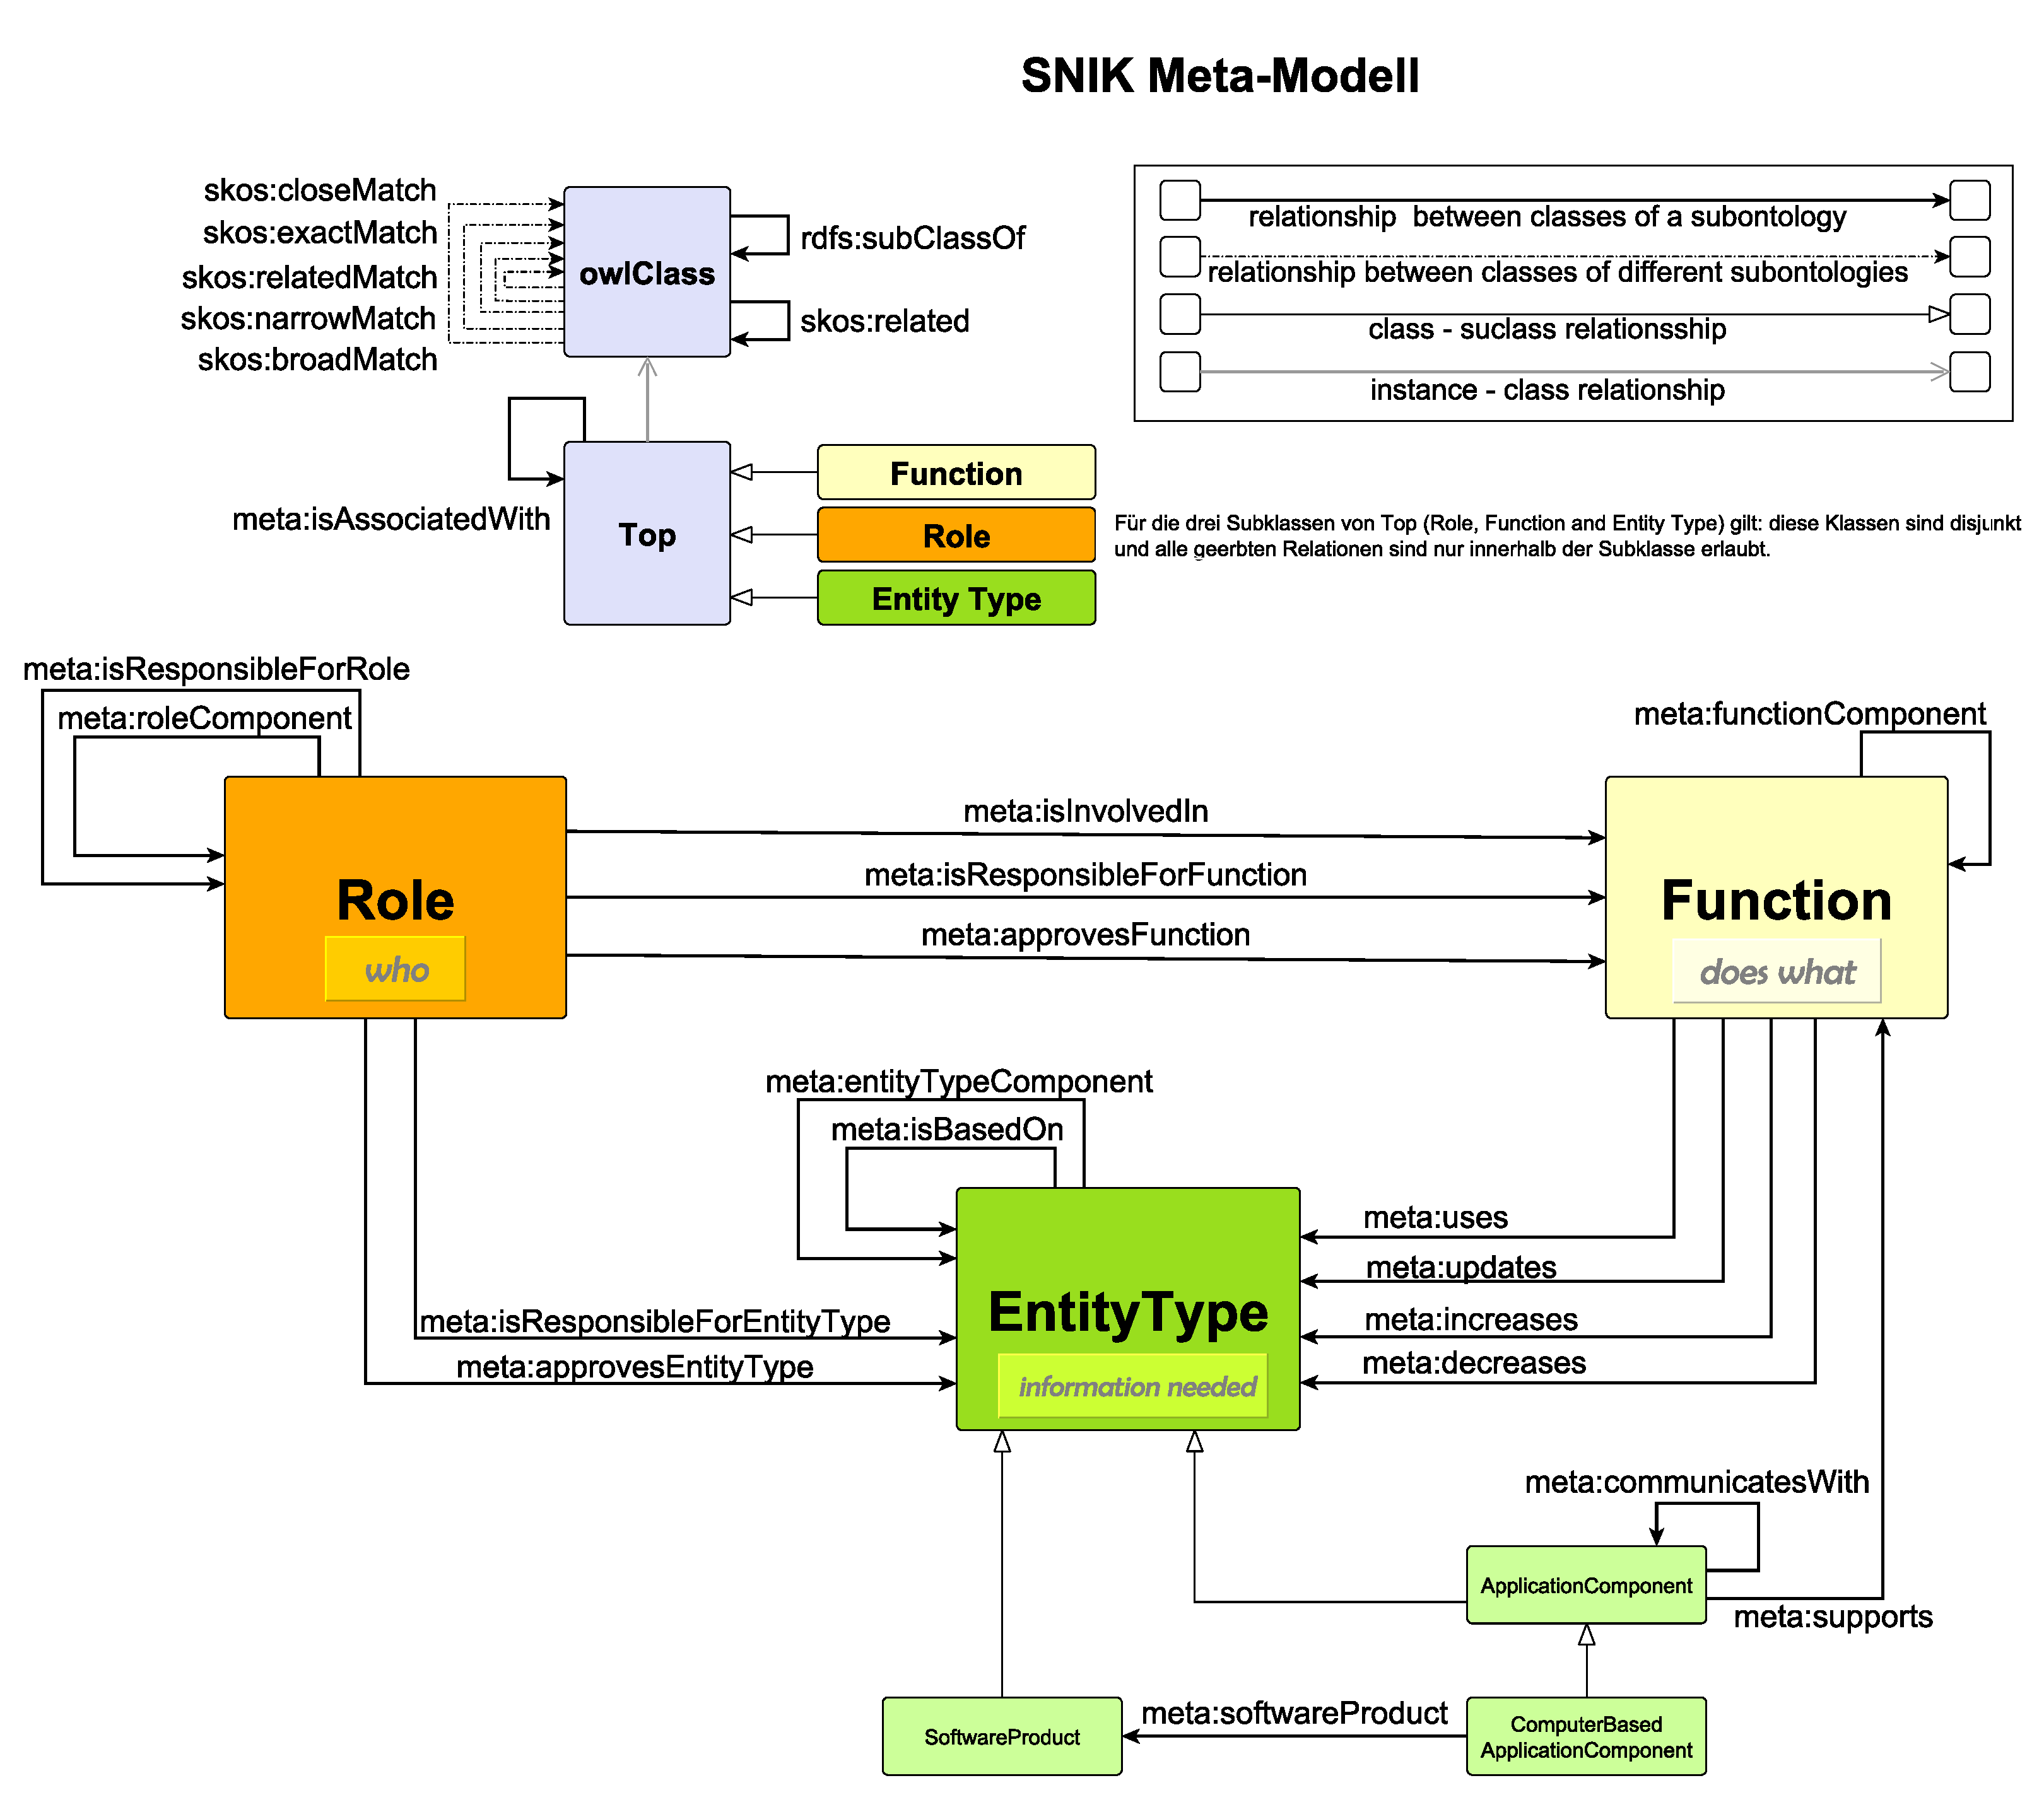
\includegraphics[width=.8\textwidth, height=.9\textheight, keepaspectratio]{Images/snik-metamodel.pdf}
\caption[SNIK Metamodell Version 8]{Das SNIK Metamodell Version 8. Quelle: \url{https://www.snik.eu/public/SNIK_Metamodell_V8.svg}}
\label{fig:snik-metamodel}
\end{sidewaysfigure}

\subsection{\enquote{Eine Ontologie von Ontologien}}

\section{Question Answering-Programme}

\subsection{gAnswer 2}

gAnswer 2 wurde von dem Wangxuan Institute of Computer Technology entwickelt und arbeitet mit Wissensbasen, um Question Answering-Aufgaben zu lösen.
Hierfür werden die Fragen in Unterfragen aufgespalten und daraus je ein Syntaxbaum erstellt.


\subsection{DeepPavlov}
DeepPavlov ist eine open-source Bibliothek zur Entwicklung von Dialogsystemen.
Es ist in \emph{Models} und \emph{Skills} organisiert.

\subsubsection{Architektur}
Ein \emph{Model} ist eine in TensorFlow\todo{erklären was tensorflow ist} implementierte Funktion einer \ac{nlp}-Pipeline,
die sowohl ein neuronales Netz als auch ein nichtneuronales oder regelbasiertes System sein kann.
Models können auch andere Models enthalten.
Ein \emph{Skill} besteht aus Models, jedoch kann er nur Zeichenketten als Ein-/Ausgabe haben.
Sie werden deshalb häufig im Dialog verwendet.
Die Models in Skills werden über einen \emph{Chainer} verbunden, der die Konfigurationsdatei einliest und so die Parameter der Models festsetzt.
Skills und Models werden gleich implementiert und unterscheiden sich nur in den Unterschiedlichen Ein- und Ausgabemöglichkeiten.
Mehrere Skills formen einen \emph{Agent}, wie in \cref{fig:deeppavlov-architektur} sichtbar ist.
Ein Agent kann die verschiedenen Skills, aus denen er besteht, in einer Unterhaltung mit dem Benutzer verwenden und zwischen ihnen wechseln.

\begin{figure}[htbp!]
\centering
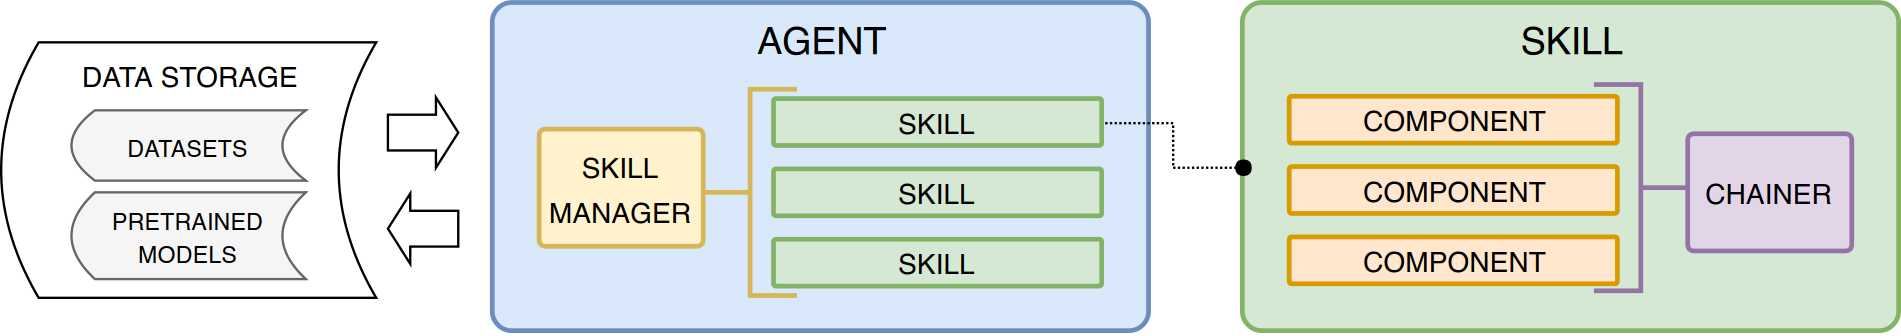
\includegraphics[width=\textwidth, height=\textheight, keepaspectratio]{Images/DeepPavlovArchitecture.png}
\caption[DeepPavlov Architektur]{Die Architektur von DeepPavlov. Quelle: \citet{deeppavlov}}
\label{fig:deeppavlov-architektur}
\end{figure}
